\documentclass[11pt]{article}
%\usepackage[firstpage]{draftwatermark}
\usepackage{times}
\usepackage{pdfpages}
\usepackage{fullpage}
\usepackage{url}
\usepackage{hyperref}
\usepackage{fancyhdr}
\usepackage{graphicx}
\usepackage{tabularx}
\usepackage{enumitem}
\usepackage{indentfirst}
\usepackage{subcaption}
\usepackage{amsmath, amsfonts, amsthm, fouriernc}
\usepackage{units}

% Added by bsb
\usepackage{color,soul}
\DeclareRobustCommand{\hlr}[1]{{\sethlcolor{red}\hl{#1}}}
\DeclareRobustCommand{\hlg}[1]{{\sethlcolor{green}\hl{#1}}}
\DeclareRobustCommand{\hlb}[1]{{\sethlcolor{blue}\hl{#1}}}
\DeclareRobustCommand{\hly}[1]{{\sethlcolor{yellow}\hl{#1}}}


\setcounter{secnumdepth}{4}
\graphicspath{{images/}}
\pagestyle{fancy}

\newenvironment{xitemize}{\begin{itemize}\addtolength{\itemsep}{-0.75em}}{\end{itemize}}
\newenvironment{tasklist}{\begin{enumerate}[label=\textbf{\thesubsubsection-\arabic*},ref=\thesubsubsection-\arabic*,leftmargin=*]}{\end{enumerate}}
\newcommand\todo[1]{{\bf TODO: #1}}
\setcounter{tocdepth}{2}
\setcounter{secnumdepth}{4}

\addtolength{\headheight}{2em}
\addtolength{\headsep}{1.5em}
\rhead{ME 2801}

\setlength\parindent{0pt}

\begin{document}

\begin{center}
  \huge{\bf ME2801, HW \#7, Root Locus, Compensation Design}
\end{center}

This assignment is two design problems via root locus for a PD and PI compensator respectively.  The exercises are verbose and intended to walk you through each step of the root locus design process.  To perform the analysis, most of the work will be done in MATLAB.  You can document the designs by following the steps and submiting the results as a MATLAB script, live script, written results or a combination.


\section{Designing compensation (P and PD) with root locus}

Consider the Plant transfer function
\[
L(s) = \frac{s+6}{(s+2)(s+3)(s+5)}
\]

\subsection{Proportional-Only Controller Design}
Consider the proportional-only, unity feedback design as shown in Figure~\ref{f:p}.
\begin{itemize}
\item Plot the root locus for the system.  Use the \texttt{sgrid()} command to add a line for $\zeta=0.707$ (\%OS=4.3).  Submit this plot.
\item Find a value for the proportional gain, $K$, so that the \emph{dominant closed-loop second order poles} have a damping ratio of approximately $\zeta = 0.707$.  Report this value of gain, $K$.
\item Using the proportional gain you found, create a closed-loop unit step response for the design and report the settling time, damping ratio and overshoot.
\end{itemize}
\begin{figure}[hbt!]
\centering  
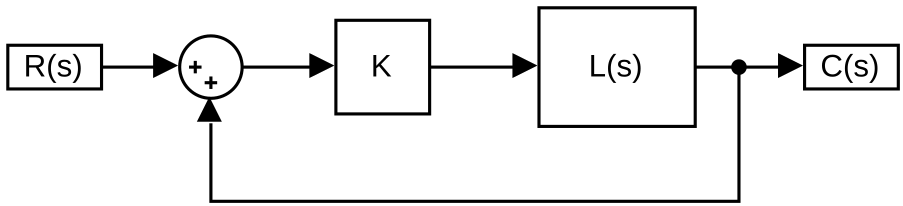
\includegraphics [width=0.6\textwidth]{p_control.png}
\caption{Proportional Control.}
\label{f:p}
\end{figure}

\subsection{Proportional-Derivative Design}
An ideal PD controller can be equivalently represented in the following forms:
\[
\begin{array}{rcll}
D(s) & = & K_p + K_d s & \text{(Standard form)} \\
  & = & K_d \left(s + {K_p}/{K_d}\right) & \text{(Factored form)} \\
  & = & K_{pd} (s + z_{pd}) & \text{(Root locus PD form)}
\end{array}
\]
where $K_p$ is the proportional gain and $K_d$ is the derivative gain in the standard form; $K_{pd}$ is the root locus gain and $z_{pd}$ is the location of the PD zero in the root locus form.  The PD controller is used to improve the transient response of the system.  The PD controller adds a zero to the system, which can be used to change the system dynamics.  The PD controller does not change the steady-state error of the system, but it can improve the transient response by increasing the damping ratio and reducing the overshoot.

Consider the PD control design shown in Figure~\ref{f:pd}. The design goal is to achieve the following closed-loop step response metrics:
\begin{itemize}
\item $T_s \approx \unit[0.9]{s}$
\item $\zeta \approx 0.707$
\end{itemize}


\begin{figure}[hbt!]
\centering  
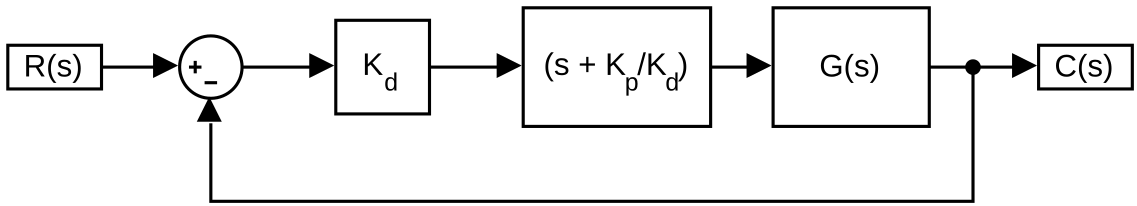
\includegraphics [width=0.6\textwidth]{pd_control.png}
\caption{Proportional-Derivative Control.}
\label{f:pd}
\end{figure}

The PD compensator design has two design parameters.   For root locus design we consider these two parameters as the location of the PD zero, $z = K_p/K_d$, and the gain value $K_d$.
\begin{itemize}
\item Find the target closed-loop pole locations that correspond to the performance metric goals, $T_s$ and $\zeta$.  That is, based on the provided metrics, what is the closed-loop, underdamped, second-order pole values (real and imaginary) to satisfy the design?  
%$s = -\zeta \omega_n \pm j \,\omega_d$, where $\omega_d = \omega_n \sqrt{1-\zeta^2}$
\item Find a location for the PD controller zero, the value of $z = K_p/K_d$ in Figure~\ref{f:pd}, so that the root locus passes through the target pole locations.  Try the following values for the zero location: $z = [-4, -7, -10]$.  For each value of $z$, plot the root locus and use the \texttt{sgrid} command to add a line for $\zeta=0.707$ (\%OS=4.3).  You can plot the root locus for each design as a separate window using the \texttt{rlocus} command or plot them all on the same axes using the \texttt{rlocusplot} command.  Which zero location enables satisfying the design constraints?  Choose one of the values for the zero location.
\item Find the value of $K_d$ that will place the dominate second order poles near the design target.  Use the interactive tool for the root locus figure window (Data tips) to choose a gain value ($K_d$) for which the closed loop poles will be within the design constraints. (If you used the \texttt{rlocusplot} command previously, you may need to generate the RL for just this system to be able to use the tool.)  
\item Using the zero location ($z$) and gain ($K_d$) you found, create a closed-loop step response for the PD design and report the settling time and overshoot.
\item Report the compensator design in the form $D(s) = K_d (s + K_p/K_d)$.
  \item Plot both closed-loop step response for both the P and PD compensator designs on the same axes and annotate your figure with the compensator values (P: $K$, PD: $K_d$ and zero location $K_p/K_d$) and the performance metrics ($T_s$ and \%OS).
\end{itemize}



\section{Design PI compensation with Root Locus}

Consider the plant transfer function
\[
G(s) = \frac{1}{(s+5)^2 (s+8)}.
\]
We might notice that this plant has \emph{Type 0} dynamics, so we anticipate it will have poor steady state error performance.
We want to design a proportional-integral (PI) compensator to improve the steady-state error.  We can write the PI controller in this form
\[
D(s) = K_p + \frac{K_i}{s} = K_i \left(\frac{s + K_p/K_i}{s}\right) = K \left(\frac{s+z}{s}\right),
\]
which illustrates that the controller adds a pole at zero and a zero at $-K_p/K_i$.

The design contraints for the problem are:
\begin{itemize}
\item $T_r \leq 0.9 \: \text{s}$
\item $\%OS \leq 2 \, \%$
\item $e_{\text{step}}(t \rightarrow \infty) = 0$
\end {itemize}


For an underdamped second-order system, the rise time can be approximated as
\[ T_r \approx \frac{1.8}{\omega_n}.
\]
for $\zeta < 0.7$.


\begin{enumerate}
\item Translate the design constraints into s-plane parameters.  Based on $T_r$ and \%OS, find the $\omega_n$ and $\zeta$ bounds for the desired pole locations to meet the design specification.
\item Plot the root locus for three different choices of PI zero location: $z = K_p/K_i = [-1, -4, -7]$.  Use the \texttt{sgrid} command to provide gridlines to illustrate the design constraints.  You can plot the root locus for each design as a separate window using the \texttt{rlocus} command or plot them all on the same axes using the \texttt{rlocusplot} command.
\item Which of the design choices for the PI zero locations enables satisfying the design constraints?   Choose one of the values for the zero location.
\item Using the zero location chosen in the previous step.   From the root locus plot, use the interactive tool (Data tips) to choose a gain value ($K$) for which the closed loop poles will be within the design constraints. (If you used the \texttt{rlocusplot} command previously, you may need to generate the RL for just this system to be able to use the tool.)  
\item With your chosen values of $K$ and $z$, find the closed-loop transfer function for your design.  
\item Verify that the closed-loop poles are in the location predicted by the root locus for your chosen value of $K$.
\item Plot the unit step response, and print closed-loop pole locations (see \texttt{pzmap} and \texttt{damp} commands) and step response metrics (\texttt{stepinfo}) to verify that the closed-loop design meets the design specification and has zero steady-state error.  Hint: Because the closed-loop system is more complex than a single second-order system with no zeros, even if your closed-loop poles are meet the s-plane constraints, the total system response metric goals.  A design that "gets close" is sufficient.
\item Report your compensator design in the form
  \[D(s) = K \frac{s+z}{s}.\]
\end{enumerate}

\end{document}


stepinfo reports the overshoot as 3.7
  The solution is not exact
 because the RL plot is only at discrete points and we chose a location on
 the root locus with a bit less damping.